\chapter{Vasculature Imaging}

\section{Introduction}

\subsection{\textit{In vivo} measures of tumour vasculature}

\section{Vascular staining}

\subsubsection{India Ink}

\begin{figure}
	\centering
	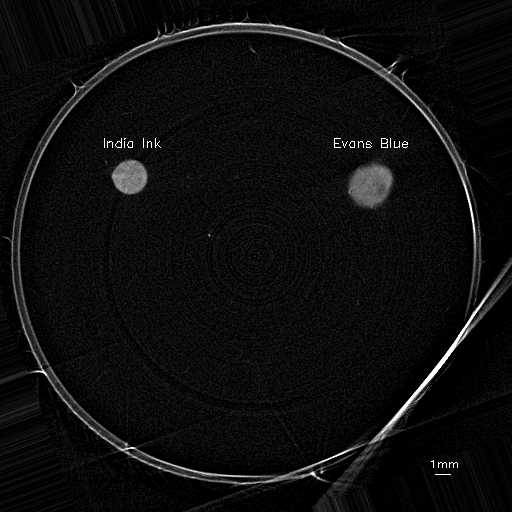
\includegraphics[width = 0.46\textwidth]{meth_img/3_EB_Ink_2mm_slice400_btscled.png}
	\caption{Phantoms with fingers containing Evans Blue, India Ink and clear gelatin.}
	\label{subfig:phant5}
\end{figure}





Figure shows that India Ink doesn't diffusive - good for staying in vessels. But Evans blue does - useful as a permeability marker.